\section{METHODS PIPELINES}
\label{METHODS PIPELINES}
%TODO merge two next paragraphs
%Performing fault detection on components is composed of two distinct problems that mussed be addressed. First, components of interest must be identified given an input image. Secondly, after successful segmentation of the respective component, its state must be classified (one of the modes of failure shown in Fig. \ref{fig:mof}). Even though a single network could be able to achieve this, a modular detection algorithm was developed, as depicted in  Fig. \ref{fig:structure}.
%Two distinct CNNs are used, one segmenting the components of interest and the second detecting faults. Utilizing two networks in serial, as shown, allows for easier implementation, as the segmentation and classification stage can be fine-tuned and trained individually. Furthermore, a modular system facilitates replacing components in the data-processing pipeline.
%
Pipeline defect detection is also composed of two problems. First, the defect should be detected, and further, it should be evaluated using segmentation results.
We propose here two different CNNs for defect detection and defect segmentation.

For image classification, we used existing architecture that achieves best results in the MFL data classification problem and proposed novel CNN architecture to compare with the existing one.
We reimplemented CNN from \cite{Feng2017} with one difference: we used squared pictures (64x64 pixels) as an input, so we didn't implement Normalization layer (first layer in the Fig.~\ref{ris:CNN_feng2017}).
\begin{figure}[ht]
	\center{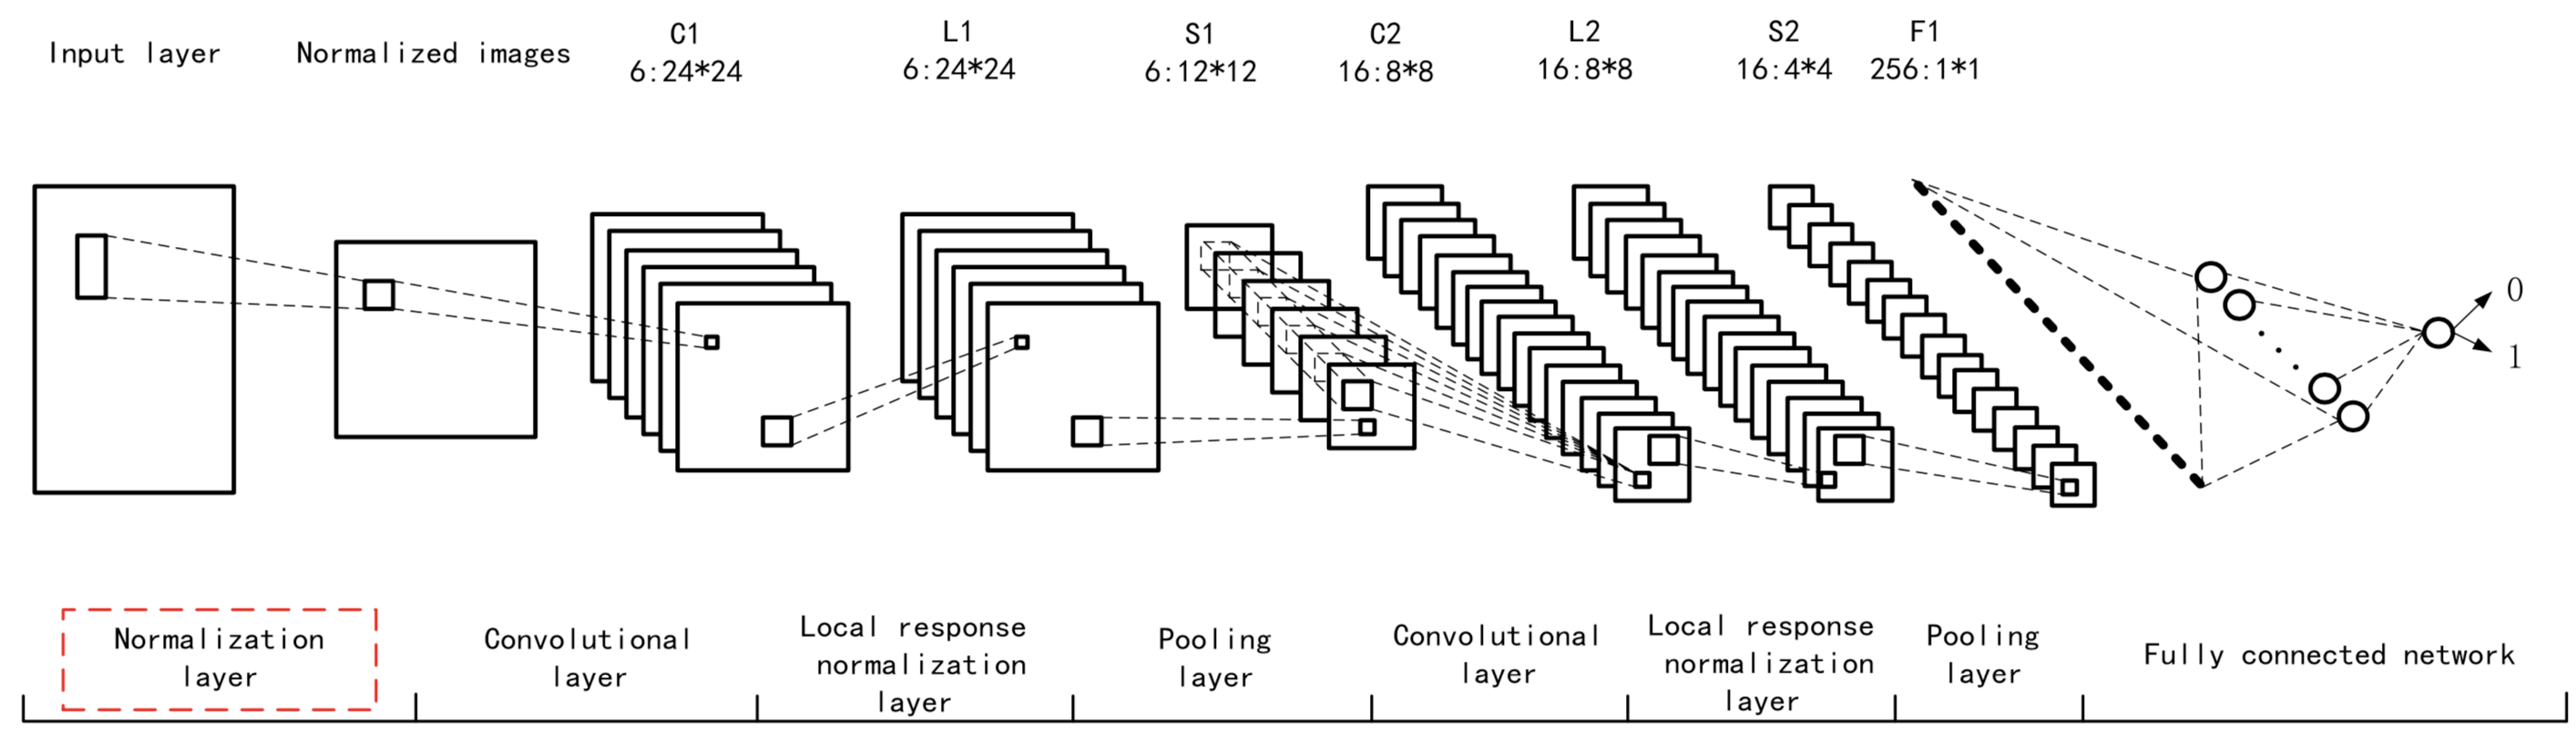
\includegraphics[scale=0.25]{pictures/CNN_feng2017.png}}
	\caption{Architecture of CNN from \cite{Feng2017}}
	\label{ris:CNN_feng2017}
\end{figure}
The interested reader can find all details and overall architecture parameters in \cite{Feng2017}.
From now on this CNN is marked as CNN-2 by the number of Convolutional layers.

Proposed model (Fig.~\ref{ris:CNN_our}) initially contains Dropout layers and Batch Normalization (BN) layers instead of Local Response Normalization (LRN) layers.
\begin{figure}[ht]
	\center{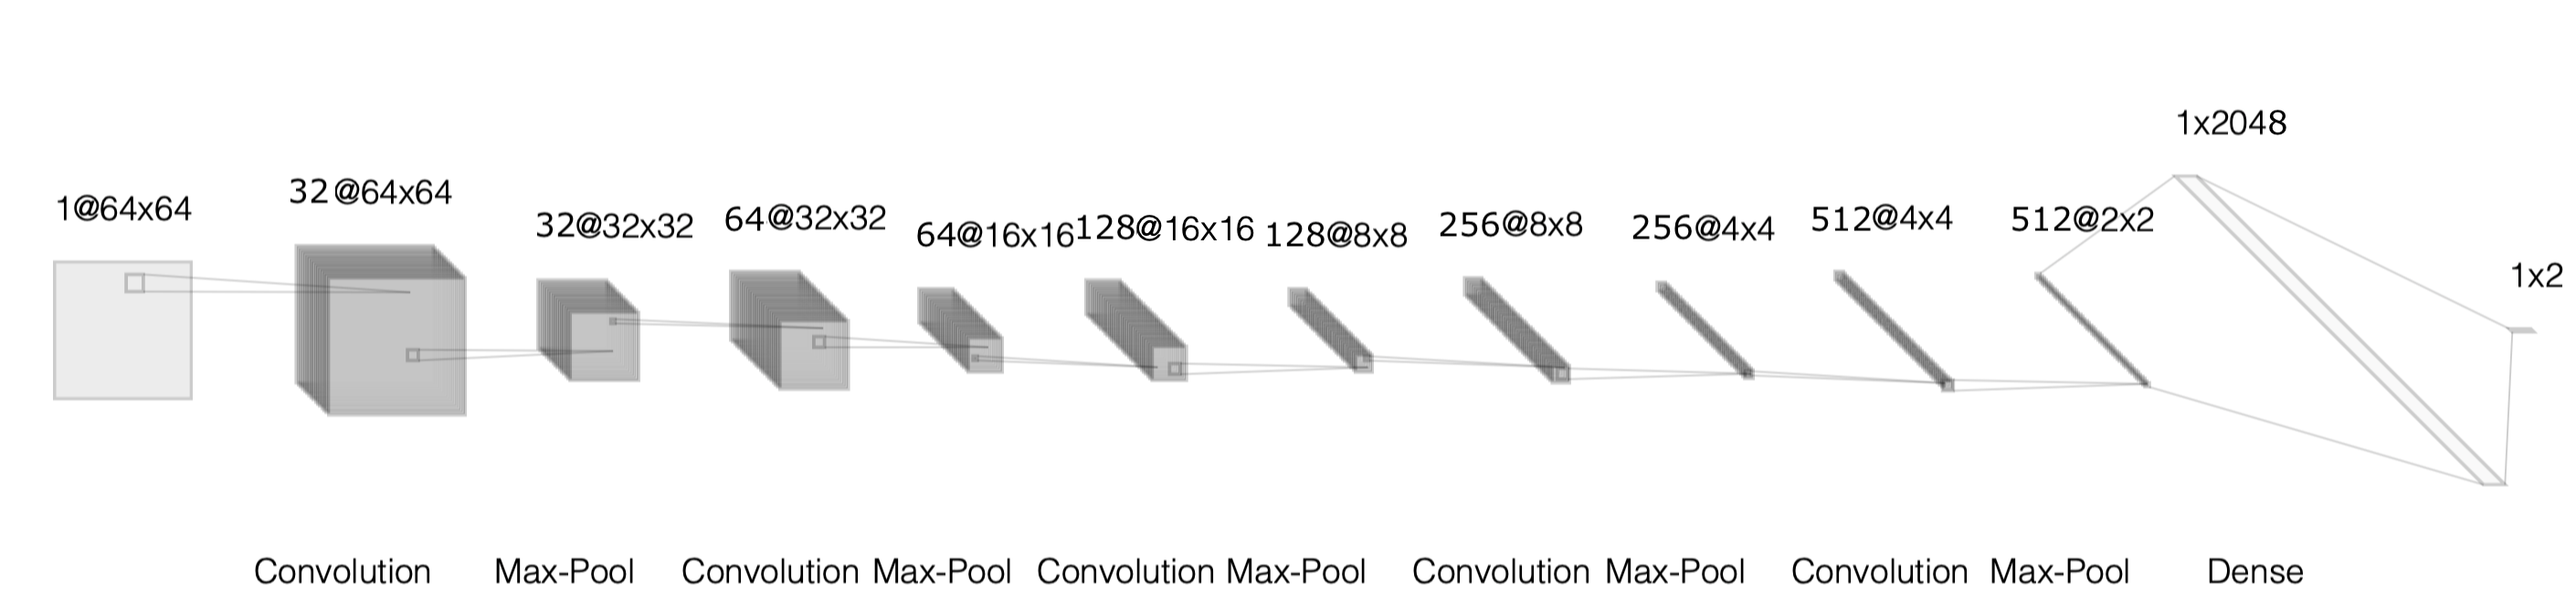
\includegraphics[scale=0.25]{pictures/CNN_our.png}}
	\caption{Architecture of the proposed CNN}
	\label{ris:CNN_our}
\end{figure}
Our model consists of 5 Convolutional layers overall.
Each Convolutional layer is followed by BN and Dropout sequentially (not shown in Fig.~\ref{ris:CNN_our}).
All Convolutional layers have equal kernel size - 5 x 5.
All MaxPooling layers have equal kernel size - 2 x 2, and stride - 2.
From now on this CNN is marked as CNN-5.

\subsection{Data and preprocessing description}
Although MFL data looks quite similar for different pipes and ILI tool types, it can differ significantly.
The data mainly depends on pipe size, wall width, sensors geometry, and other geometric characteristics.
Moreover, ILI tools differ a lot for different pipe sizes.
Therefore, the repeatability of the results for different datasets should be investigated additionally.
Following, we provide dataset characteristics.
We have data collected from the 219 mm in diameter pipe.
MFL dataset provides information about a single inspection tool run.
Dataset has 64 features collected as an array with a constant step along with the ILI tool movement inside the pipe.
Dataset has 4470704 samples that represent 15162.85 meters long pipeline part.
Sample values vary from 0 to 4095 units.
It has 745 defects of different types and 1462 welds, 34 of which are defected.
Fig.~\ref{ris:defect_example} shows examples of normal data, data with a weld, and with a defect.
Attached to the dataset technical report contains information about welds and defects location, defects types, sizes, and other related characteristics.
\begin{figure}[ht]
	\center{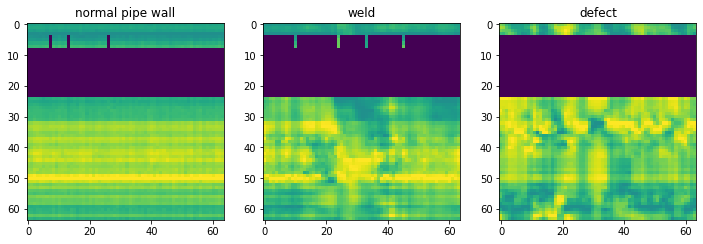
\includegraphics[scale=0.55]{pictures/1.png}}
	\caption{Example of the MFL data}
	\label{ris:defect_example}
\end{figure}

Raw data has several issues that don't allow us to solve CV problems without proper preprocessing.
They are:
\begin{enumerate}
	\item Sensors malfunctions (zeroed values cause bold horizontal line in Fig.~\ref{ris:defect_example});
	\item Displaced origins between data and reports coordinates;
	\item Inaccurate annotations, e.g., missed defects, wrong defect location, etc.
	\item No annotated data for the segmentation task.
\end{enumerate}

\subsubsection{Sensors malfunctions problem}
To deal with sensors malfunctions we suppose to fill the gaps (zeroed values) with values calculated by different methods.
Additionaly, we will consider values less than 2000 abnormal and replace them with zeroes during the preprocessing.
\begin{enumerate}
	\item Abnormal values are equal to 0. Then Min-Max scaling to $[0.5:1]$ range.
	\item Abnormal values are equal to the mean of normal values from one picture. Then Min-Max scaling.
	\item Abnormal values are equal to the mean of normal values over the column. Then Min-Max scaling.
	\item Abnormal values are equal to the mean of neighboring sensors over the column. Then Min-Max scaling.
	\item Abnormal values are equal to the interpolation results over the column. Then Min-Max scaling.
	\item Rerange initial set of values to 0...255 uint8 range.
	\item Rerange initial set of values to 0...1 float range \\ 
	(Fig.~\ref{ris:preproc_fun}). Such a specific function due to the range of normal operation of the sensor from 2500 to 3500 units.
\end{enumerate}

\begin{figure}[ht]
	\center{\includegraphics[scale=0.22]{pictures/preproc_fun.png}}
	\caption{The function for converting the initial values of signal to the input of network}
	\label{ris:preproc_fun}
\end{figure}

The results of all applied methods are presented in Fig.~\ref{ris:filling_example}.
\begin{figure}[ht]
	\center{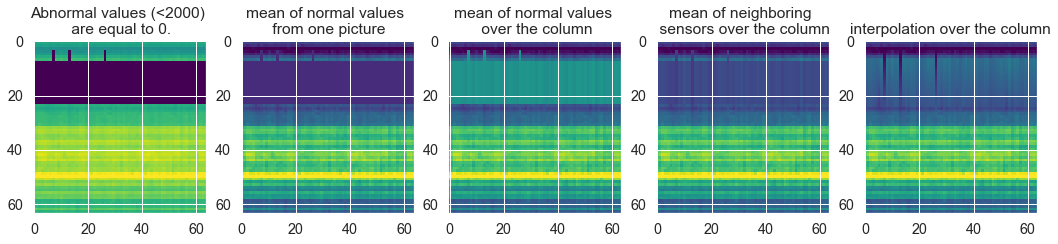
\includegraphics[scale=0.37]{pictures/2.png}}
	\caption{Comparison of missing values filling methods}
	\label{ris:filling_example}
\end{figure}

Min-Max scaling can be applied using whole dataset or just one image.
Both approaches will be compared during the experiment conducting.

Since the ILI tool location data did not match the defect location data from the report, it was necessary to merge the data. The key factor here turned out to be that signal values from magnetic flux sensors grow at the weld site (Figure \ref{ris:prepr}). 

\begin{figure}[!h]
	\center{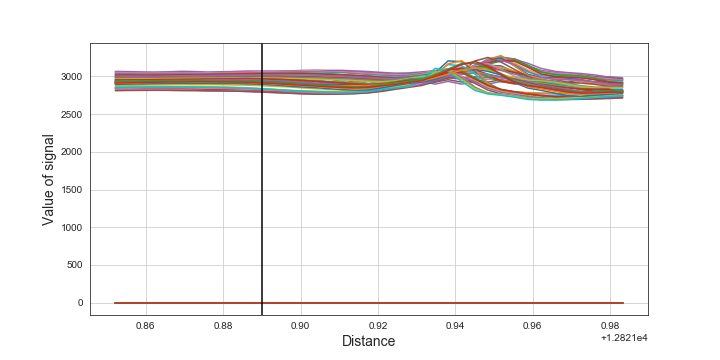
\includegraphics[width=0.8\linewidth]{pipes/prepr.png}}
	\caption{Location of a weld. The black vertical line is a weld, according to the report. Other lines are values from sensors.}
	\label{ris:prepr}
\end{figure}
The solution was to find the locations of the maxima of sensors data values and then to combine it with the weld coordinates.

\subsubsection{Manual annotations for the segmentation task}
Since there was no annotated data for the segmentation problem, it was necessary to annotate it manually (Figure \ref{ris:annot}). The characteristics of the obtained dataset can be seen in table \ref{tab:alg1}.

\begin{figure}[ht]
	\center{\includegraphics[scale=0.50]{pictures/annot.png}}
	\caption{The methodology for obtaining the mask}
	\label{ris:annot}
\end{figure}

\subsubsection{Inaccurate annotations problem}
This problem is a common one for oil and gas pipeline nondestructive testing \cite{Khodayari-Rostamabad2009}.
It appears to be a lot of missing defects that affect the quality of the problem.
Besides, there are wrong defect types and locations.
To eliminate wrong location issue, we additionaly searched extremums around the provided location and chose the defects or welds taking into account new coordinates.

\subsubsection{Augmentation}
Although we have a lot of data, we don't have a lot of defects and welds in comparison with normal pipe wall instances.
We use the augmentation procedure to balance classes of pictures and increase the model's quality by increasing the number of instances in small classes (defects, welds).
As an augmentation tool we use Albumentations library \cite{buslaev2020albumentations}.
For welds pictures we apply following augmentations:
\begin{enumerate}
	\item Rotate (limit=180, p=1),
	\item VerticalFlip (p=1), 
	\item HorizontalFlip (p=1), 
	\item ElasticTransform (p=1, alpha=20, sigma=120 * 0.05, alpha affine=120 * 0.03), 
	\item GridDistortion (p=1),
	\item OpticalDistortion (p=1, distort limit=2, shift limit=0.5).
\end{enumerate}

And for defects we apply following ones:
\begin{enumerate}
	\item Transpose (p=1), 
	\item Rotate (limit=90, p=1), 
	\item Rotate (limit=180, p=1), 
	\item Rotate (limit=270, p=1,), 
	\item VerticalFlip (p=1), 
	\item HorizontalFlip (p=1), 
	\item ElasticTransform (p=1, alpha=20, sigma=120 * 0.05, alpha affine=120 * 0.03),
	\item RandomRotate90 (p=1),
	\item GridDistortion (p=1),
	\item OpticalDistortion (p=1, distort limit=1, shift limit=0.3).
\end{enumerate}
Examples of augmentations are shown in Fig.~\ref{ris:aug_example}.
\begin{figure}[ht]
	\center{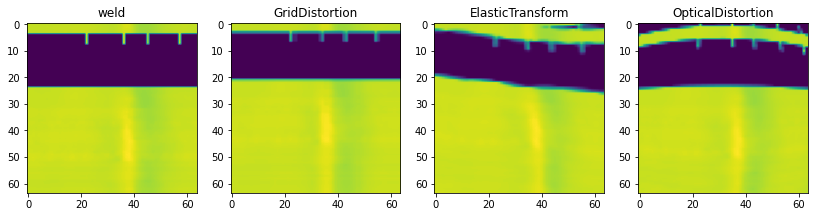
\includegraphics[scale=0.55]{pictures/4.png}}
	\caption{Examples of the augmentation results}
	\label{ris:aug_example}
\end{figure}


The characteristics of the pipeline defects dataset are described in Table \ref{tab:alg1}, where * symbol indicates a random call function 5 and 6 from the defects augmentation list, so the exact number is unknown.
\begin{table}[!htb]
	\caption{\label{tab:alg1}Dataset size for pipeline defects detection and segmentation problems}
	\begin{center}
		\small
		\begin{tabular}{| c | c  c  c | c  c |}
			\multicolumn{1}{c}{} & \multicolumn{3}{c}{Classification} & \multicolumn{2}{c}{Segmentation} \\
			\hline
			Data & Normal & Defect & Weld & Normal & Defect \\
			\hline
			\multicolumn{6}{|c|}{Before augmentation}  \\
			\hline
			Train  & 11106 & 569 & 1130 & 181 & 450 \\
			Validation & 584 & 142 & 282 & 33 & 111 \\
			\hline
			\multicolumn{6}{|c|}{After augmentation}  \\
			\hline
			Train  & 11106 & 8535 & 11300 & * & * \\
			Validation & 584 & 142 & 282 & * & * \\
			\hline
		\end{tabular}
	\end{center}
\end{table}

\subsection{Performance metrics}
For the classification problem we use Accuracy.
Accuracy is defined by the formula:
$$Acc = \frac{\sum_{i=0}^{N} 1_{\{\hat{y}_i=y_i\}}}{N},$$
where $N$ - number of samples, $\hat{y}$ - predicted label, $y$ - true label.
